\begin{frame}{Pump--probe：双场展开与最低三阶响应}

  \footnotesize
  \setlength{\abovedisplayskip}{1.5pt}
  \setlength{\belowdisplayskip}{1.5pt}

  \begin{columns}[c,onlytextwidth]
    \begin{column}{0.62\textwidth}
      \[
        \alpha(t)=\sum_{n,m}\eta_p^n\eta_{p'}^m
          \alpha^{(n)(m)}(t),
        \qquad
        \rho(t)=\sum_{n,m}\eta_p^n\eta_{p'}^m
          \rho^{(n)(m)}(t).
      \]
      {\centering
        $(n,m)=(\text{pump 阶数},\,\text{probe 阶数})$。\par}
    \end{column}
    \begin{column}{0.36\textwidth}
      {\centering
        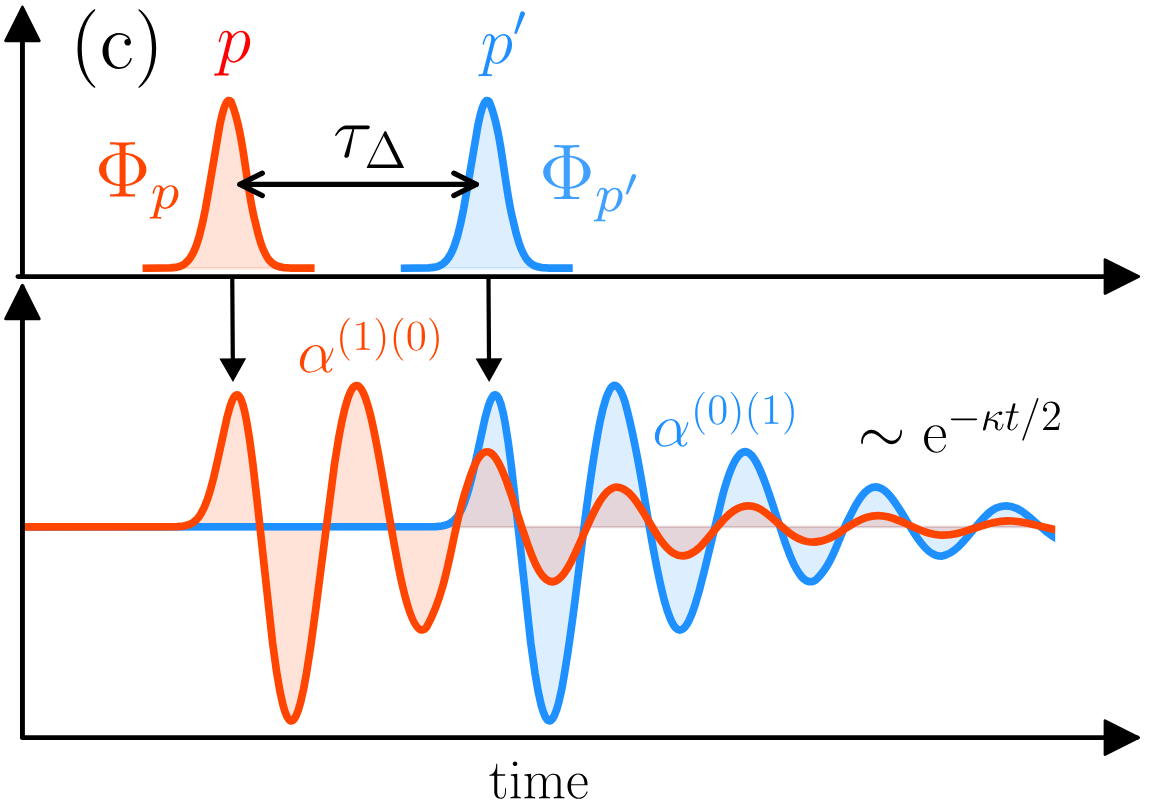
\includegraphics[width=0.76\linewidth,keepaspectratio]{../ref/fig1c.png}\par}
      {\centering\tiny\color{gray}
        $\tau_\Delta=\tau_{p'}-\tau_p$：pump 先作用，probe 延迟读取。\par}
    \end{column}
  \end{columns}

  \vspace{0.1em}

  {\centering\small
    相同二能级分子系综 + 单模腔
    $\xrightarrow{\;G=g\sqrt N\;}$ LP/UP。\par}
  {\centering\tiny\color{gray}
    pump 使体系偏离平衡，probe 延迟读取瞬态响应。\par}

  \vspace{0.15em}

  \begin{center}
  \begin{tikzpicture}[>=stealth,
      every node/.style={inner sep=2pt}]
    \node (r0) {$\rho^{(0)}$};
    \node (r1) at (3.1,0) {$\rho^{(1)(0)}$};
    \node (r2) at (6.2,0) {$\rho^{(2)(0)}$};
    \node (r3) at (9.3,0) {$\rho^{(2)(1)}$};
    \draw[->] (r0) -- node[above,font=\scriptsize]{\textcolor{Plum}{$p$}}
      node[below,font=\scriptsize]{相干} (r1);
    \draw[->] (r1) -- node[above,font=\scriptsize]{\textcolor{Plum}{$p$}}
      node[below,font=\scriptsize]{布居} (r2);
    \draw[->] (r2) -- node[above,font=\scriptsize]{\textcolor{NavyBlue}{$p'$}}
      node[below,font=\scriptsize]{读取} (r3);
    \draw[rounded corners=3pt,thin,black!50]
      ([xshift=-8pt,yshift=-5pt]current bounding box.south west)
      rectangle
      ([xshift=8pt,yshift=5pt]current bounding box.north east);
  \end{tikzpicture}
  \end{center}

  \vspace{0.2em}

  {\centering
    $p^2p'\ \Longrightarrow\ \alpha^{(2)(1)}$，\qquad
    这是二能级示例中的最低三阶 pump--probe 响应。\par}

  \papersource{Reitz, Koner \& Yuen-Zhou, PRL 134, 193803 (2025), Eq.~(6), Fig.~1(c).}

\end{frame}

\begin{frame}{差分透射谱}

  \footnotesize
  \setlength{\abovedisplayskip}{2pt}
  \setlength{\belowdisplayskip}{2pt}

  \begin{columns}[c,onlytextwidth]
    \begin{column}{0.48\textwidth}
      {\centering\fboxsep=5pt\fboxrule=0.4pt
      \fbox{\begin{minipage}{0.92\linewidth}
        {\centering\textbf{pump off}\par}
        \[
          \text{弱 probe}
          \rightarrow\alpha^{(0)(1)}(\omega)
          \rightarrow T_{\rm off}(\omega)
        \]
        {\centering\scriptsize
          线性基准：对应第一篇中的弱探测线性透射。\par}
      \end{minipage}}\par}
    \end{column}
    \begin{column}{0.48\textwidth}
      {\centering\fboxsep=5pt\fboxrule=0.4pt
      \fbox{\begin{minipage}{0.92\linewidth}
        {\centering\textbf{pump on}\par}
        \[
          \text{pump + probe}
          \rightarrow\alpha(\omega,\tau_\Delta)
          \rightarrow T_{\rm on}(\omega,\tau_\Delta)
        \]
        {\centering\scriptsize
          pump 改变体系后得到的瞬态探测透射。\par}
      \end{minipage}}\par}
    \end{column}
  \end{columns}

  \vspace{0.3em}

  \[
    T_{p'}(\omega)
    =\left|
      \frac{(\kappa/2)\,\alpha(\omega)}{\eta_{p'}f_{p'}(\omega)}
    \right|^2
    \qquad
    \Delta T(\omega,\tau_\Delta)
    =T_{\rm on}-T_{\rm off}
  \]
  {\centering\scriptsize\color{gray}
    二者都通过同一标准输入--输出关系由腔内场得到；
    区别只在于 pump on/off 时的腔内场不同。\par}

  \vspace{0.2em}

  {\centering\scriptsize
    $\Delta T>0$：透射增强；\qquad $\Delta T<0$：透射减弱。\par
    因此差分透射测量的是 pump 对原线性 probe 光谱的改变量。\par}

  \vspace{0.3em}

  \[
    \physmark{OliveGreen}{dtResult}{\Delta T^{(3)}(\omega)}
    \propto2\operatorname{Re}\!\left[
      \physmark{NavyBlue}{dtLO}{\alpha^{(0)(1)*}(\omega)}
      \physmark{Plum}{dtNL}{\alpha^{(2)(1)}(\omega)}
    \right].
  \]
  {\centering\scriptsize
    由于探测器测量强度 $T\propto|\alpha|^2$，
    线性 probe 场与三阶场的交叉项给出最低阶差分透射信号。\par}
  {\centering\tiny\color{gray}
    $\alpha^{(0)(1)}$：线性 probe 基准场；\quad
    $\alpha^{(2)(1)}$：pump 诱导的三阶场。\par}

  \papersource{PRL Eqs.~(7)--(8); SM Eqs.~(S.11)--(S.14).}

\end{frame}

\begin{frame}{Fig.~3：差分透射读取相干与布居的时间尺度}

  \footnotesize

  \begin{columns}[c,onlytextwidth]
    \begin{column}{0.61\textwidth}
      {\centering
        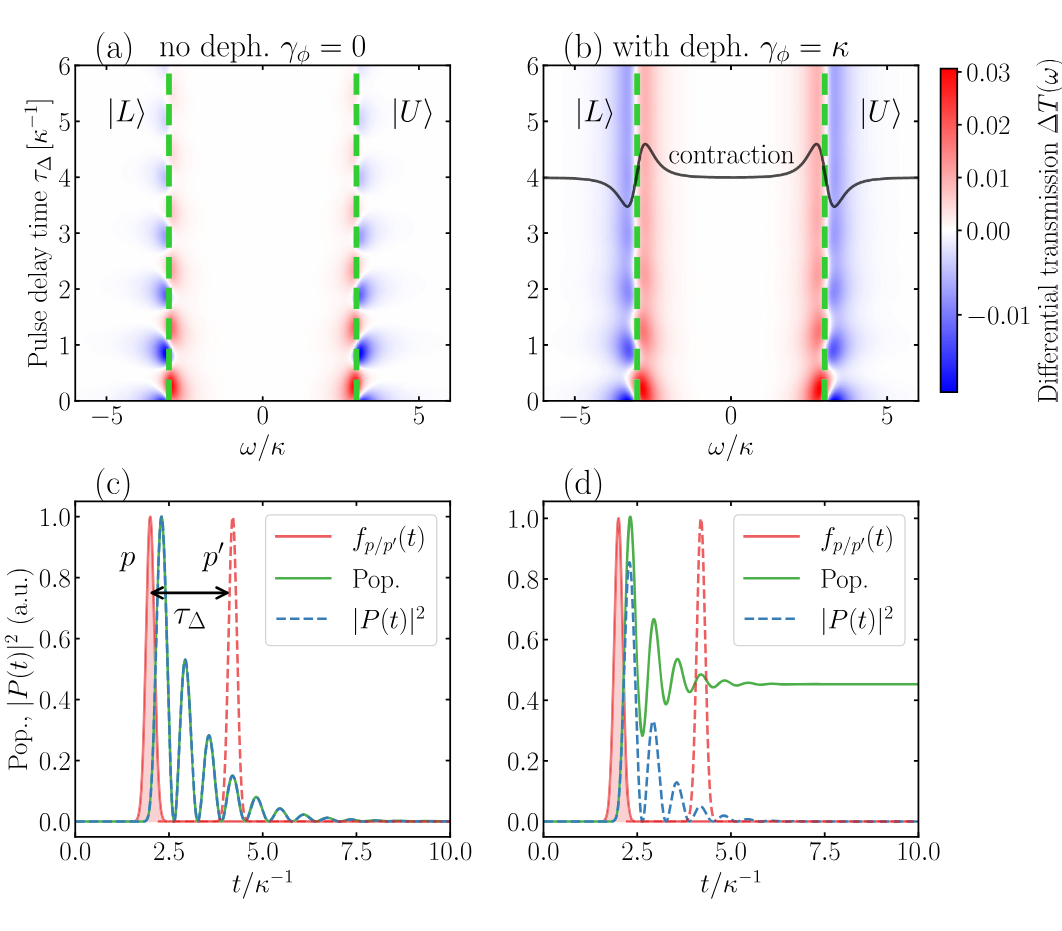
\includegraphics[width=0.85\linewidth,keepaspectratio]{../ref/fig3.png}\par}
    \end{column}
    \begin{column}{0.37\textwidth}
      {\scriptsize\color{gray}
        红：$\Delta T>0$，
        \\
        蓝：$\Delta T<0$；
        \\
        绿虚线：LP/UP 共振位置。\par}

      \vspace{0.6em}
      \textbf{(c)$\rightarrow$(a)，$\gamma_\phi=0$}\par
      {\scriptsize
        相干与布居振荡导致 UP--LP 相位拍频，
        因此 $\Delta T$ 随延迟出现红蓝交替条纹。\par}

      \vspace{0.6em}
      \textbf{(d)$\rightarrow$(b)，$\gamma_\phi=\kappa$}\par
      {\scriptsize
        退相使相干迅速衰减，但布居仍可保留，
        因此时间条纹消失，而长延迟下仍可见谱修正与劈裂收缩。\par}

    \end{column}
  \end{columns}

  \papersource{Original PRL Fig.~3(a--d), p.~193803-4; SM Eq.~(S.14), Fig.~S1.}

\end{frame}
